\graphicspath{ {images/student/} }

\section{Студенты}

Раздел \quotes{Студенты} содержит в себе функции по работе со студентами: загрузку студентов на Платформу, зачисление, 
отчисление, изменение режима прохождения сессии курса.

\subsection{Роли и операции}
Раздел доступен пользователям, имеющим следующие роли:
\begin{itemize}
	\item Администратор Платформы:
	\begin{itemize}
		\item загрузка студентов списком;
		\item просмотр списка студентов вуза;
		\item просмотр подробной информации о студенте вуза;
		\item создание и редактирование заявки на зачисление;
		\item просмотр подробной информация о заявке на зачисление;
		\item создание заявки на изменение режима прохождения сессии курса;
		\item просмотр подробной информация о заявке на изменение режима прохождения сессии курса;
		\item создание заявки на зачисление;
		\item создание заявки на зачисление списком;
		\item отчисление студентов;
		\item изменение режима прохождения сессии курса студентами;
		\item создание заявки на изменение режима прохождения сессии курса;
		\item создание заявки на изменение режима прохождения сессии курса списком.
	\end{itemize}
	\item Администратор вуза"=поставщика:
	\begin{itemize}
		\item загрузка студентов списком;
		\item просмотр студентов, обучающихся на курсах вуза;
		\item зачисление студентов;
		\item отчисление студентов;
		\item изменение режима прохождения сессии курса студентами;
		\item зачисление студентов списком.
	\end{itemize}
	\item Администратор вуза"=потребителя:
	\begin{itemize}
		\item загрузка студентов списком;
		\item просмотр списка студентов вуза;
		\item просмотр подробной информации о студенте вуза;
		\item создание и редактирование заявки на зачисление;
		\item просмотр подробной информация о заявке на зачисление;
		\item создание заявки на изменение режима прохождения сессии курса;
		\item просмотр подробной информация о заявке на изменение режима прохождения сессии курса;
		\item создание заявки на зачисление;
		\item создание заявки на зачисление списком;
		\item создание заявки на изменение режима прохождения сессии курса;
		\item создание заявки на изменение режима прохождения сессии курса списком.
	\end{itemize}
\end{itemize}

%Данный раздел доступен пользователям с ролями: 
%администратор вуза"=поставщика, администратор вуза потребителя и администратор Платформы.

%Для администратора вуза"=поставщика доступны следующие пункты меню:
%\begin{itemize}
%	\item загрузка студентов списком;
%	\item обучающиеся на курсах вуза;
%	\item зачисление студентов;
%	\item отчисление студентов;
%	\item изменение режима прохождения сессии курса студентами;
%	\item зачисление студентов списком.
%\end{itemize}

%Для администратора вуза"=потребителя доступны следующие пункты меню:
%\begin{itemize}
%	\item загрузка студентов списком;
%	\item студенты вуза;
%	\item подробная информация о студенте вуза;
%	\item заявки на зачисление;
%	\item подробная информация о заявке на зачисление;
%	\item заявки на изменение режима прохождения сессии курса;
%	\item подробная информация о заявке на изменение режима прохождения сессии курса;
%	\item создание заявки на зачисление;
%	\item создание заявки на зачисление списком;
%	\item создание заявки на изменение режима прохождения сессии курса;
%	\item создание заявки на изменение режима прохождения сессии курса списком.
%\end{itemize}

%Администратору Платформы доступны все вышеперечисленные пункты меню.

\subsection{Загрузка студентов списком}

Внешний вид формы загрузки студентов списком представлен на рис.~\ref{img:student:mass_invite}. 
Для осуществления загрузки студентов списком необходимо нажать на кнопку \quotes{Обзор} и в появившемся диалоге 
выбрать CSV"=файл с заголовками {\tt email}, {\tt last\_name}, {\tt first\_name}, {\tt username} и данными о студентах. 
Шаблон требуемого файла можно скачать, нажав на ссылку \quotes{Скачать шаблон}.

\begin{figure}[H]
	\center{
\includegraphics[width=1\linewidth]{mass_invite}}
	\caption{Загрузка студентов списком}
	\label{img:student:mass_invite}
\end{figure}

После выбора файла необходимо нажать на кнопку \quotes{Загрузить}, после чего начнется загрузка файла и его обработка.
При загрузке некорректного файла могут отобразиться следующие ошибки:
\begin{itemize}
	\item в CSV"=файле отсутствуют столбцы {\tt email}, {\tt last\_name}, {\tt first\_name}, {\tt username};
	\item CSV"=файл пустой.
\end{itemize} 

При загрузке корректного файла результаты обработки отображаются в виде двух таблиц: 
первая таблица содержит данные об успешно зарегистрированных студентах, 
вторая таблица содержит данные о незарегистрированных студентах с указанием ошибок. 
Все успешно загруженные студенты ассоциируются с вузом, из кабинета которого были загружены.
Результат загрузки студентов представлен на рис.~\ref{img:student:mass_invite_result}.

\begin{figure}[H]
	\center{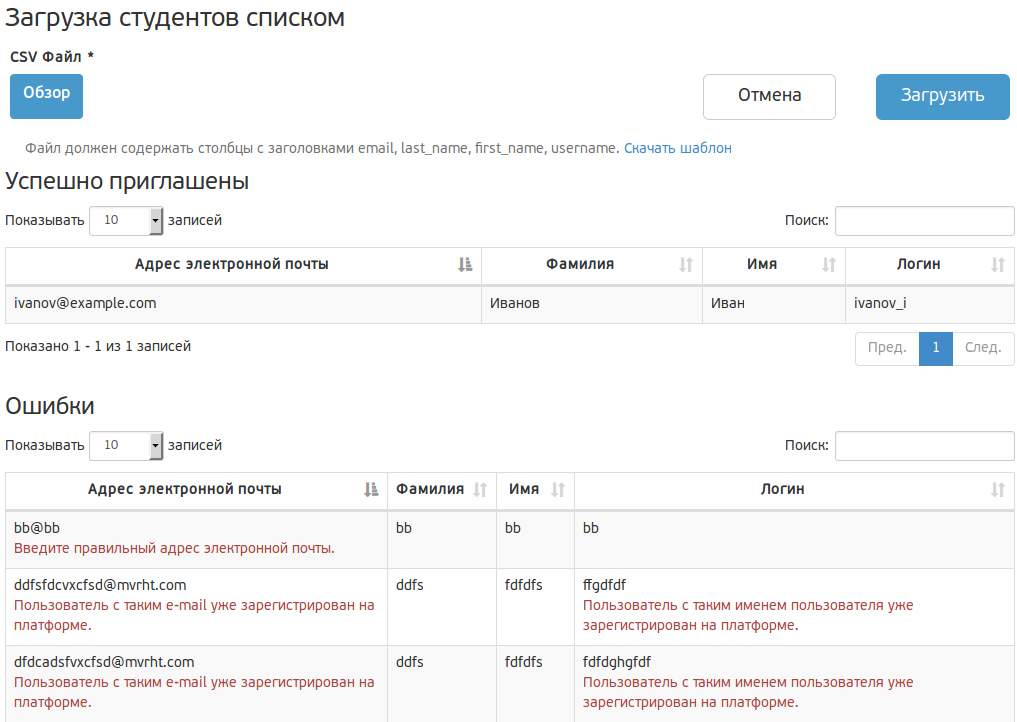
\includegraphics[width=1\linewidth]{mass_invite_result}}
	\caption{Результат загрузки студентов списком}
	\label{img:student:mass_invite_result}
\end{figure}

\subsection{Обучающиеся на курсах вуза}
Список студентов, обучающихся на курсах вуза "--- это табличное представление всех студентов, 
проходящих обучение на какой"=либо сессии курса данного вуза.
Внешний вид списка представлен на рис.~\ref{img:student:enrolled_list}. 
Элементы управления табличными представления описаны в подразделе~\ref{sec:datatables}.
Таблица содержит следующие столбцы:
\begin{itemize}
	\item ФИО студента;
	\item сессии курсов данного вуза, на которые зачислен студент;
	\item активность;
	\item успеваемость.
\end{itemize}

\begin{figure}[H]
	\center{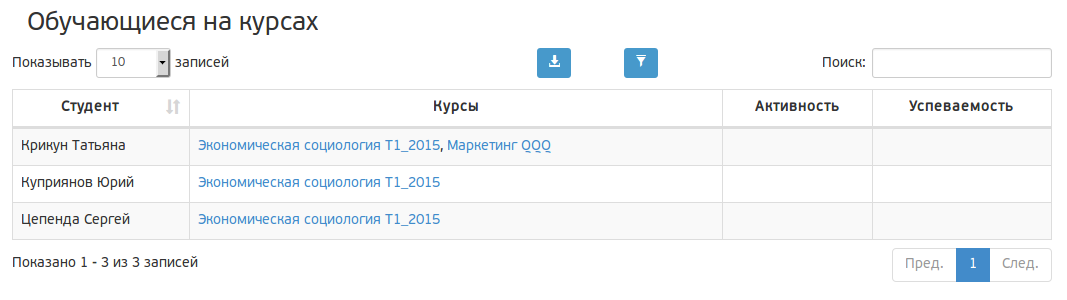
\includegraphics[width=1\linewidth]{enrolled_list}}
	\caption{Список студентов, обучающихся на курсах вуза}
	\label{img:student:enrolled_list}
\end{figure}

Внешний вид диалога фильтрации списка студентов представлен на рис.~\ref{img:student:enrolled_list_filter}.
Можно фильтровать список по следующим полям:
\begin{itemize}
	\item ФИО студента "--- текстовое поле;
	\item курс, на сессию которого он зачислен "--- виджет выпадающего списка с автодополнением с возможностью 
	множественного выбора (описание виджета см. в подразделе~\ref{widget:autocomplete_with_multiselect}).
\end{itemize}

\begin{figure}[H]
	\center{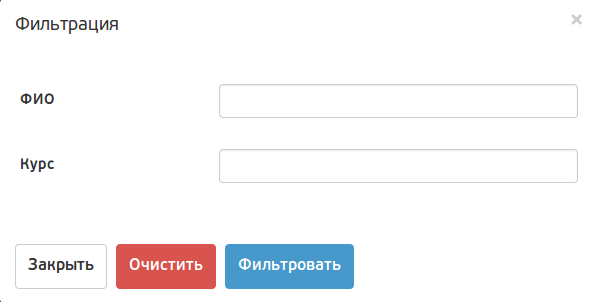
\includegraphics[height=5.5cm]{enrolled_list_filter}}
	\caption{Диалог фильтрации списка студентов, обучающихся на курсах вуза}
	\label{img:student:enrolled_list_filter}
\end{figure}

\subsection{Зачисление студентов}
Внешний вид формы зачисления студентов представлен на рис.~\ref{img:student:enroll}. 

\begin{figure}[H]
	\center{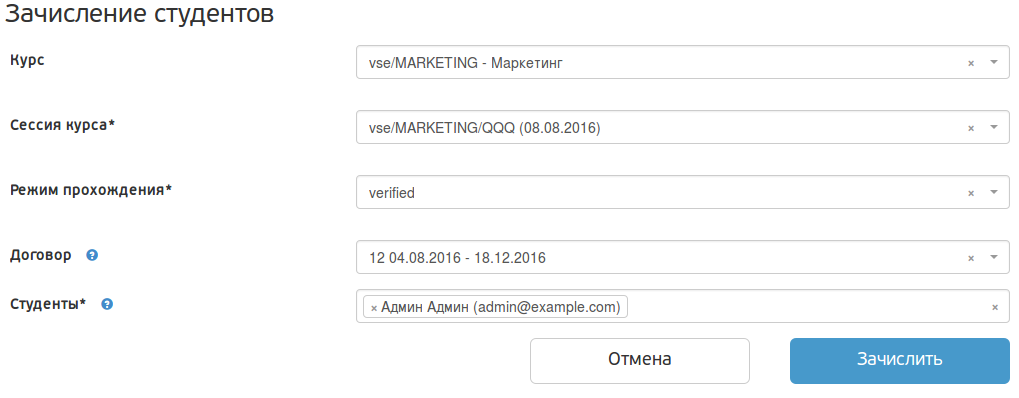
\includegraphics[width=1\linewidth]{enroll}}
	\caption{Зачисление студентов на сессию курса}
	\label{img:student:enroll}
\end{figure}

Для зачисления студентов необходимо:
\begin{enumerate}
	\item в выпадающем списке с автодополнением выбрать курс, который будут проходить студенты 
	(описание виджета см. в подразделе~\ref{widget:autocomplete});
	\item в выпадающем списке с автодополнением выбрать конкретную сессию этого курса 
	(описание виджета см. в подразделе~\ref{widget:autocomplete});
	\item в выпадающем списке с автодополнением выбрать один из режимов прохождения, доступных в рамках выбранной сессии 
	(описание виджета см. в подразделе~\ref{widget:autocomplete});
	\item опционально можно в выпадающем списке с автодополнением выбрать договор с вузом"=потребителем, 
	по которому осуществляется зачисление студентов (описание виджета см. в подразделе~\ref{widget:autocomplete});
	\item выбрать одного или нескольких студентов из числа уже зарегистрированных пользователей на Платформе при помощи 
	виджета выпадающего списка с автодополнением с возможностью множественного выбора 
	(описание виджета см. в подразделе~\ref{widget:autocomplete_with_multiselect}). 
\end{enumerate}

Изначально поля выбора договора и студентов неактивны, они активируются только после выбора сессии курса.
После выбора курса в выпадающем списке сессий будут перечислены только сессии выбранного курса, 
а в списке договоров "--- только договоры, заключенные для этого курса.
После выбора сессии курса в списке студентов будут перечислены только студенты, 
которые еще не зачислены на выбранную сессию курса.
В случае выбора режима <<verified>> (с подтверждением личности), поле <<договор>> становится обязательным для заполнения. 


В случае, если заполнено поле договора с вузом"=потребителем и количество свободных мест по договору меньше, 
чем количество выбранных для зачисления студентов, система выдаст предупреждение 
(рис.~\ref{img:student:enroll_student_error}), но на возможность зачисления студентов оно не влияет.

\begin{figure}[H]
	\center{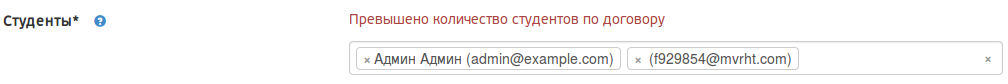
\includegraphics[width=1\linewidth]{enroll_student_error}}
	\caption{Превышение количества студентов по договору.}
	\label{img:student:enroll_student_error}
\end{figure}

После заполнения всех полей необходимо нажать на кнопку \quotes{Зачислить}.

\subsection{Отчисление студентов}
Внешний вид формы отчисления студентов представлен на рис.~\ref{img:student:unenroll}. 

\begin{figure}[H]
	\center{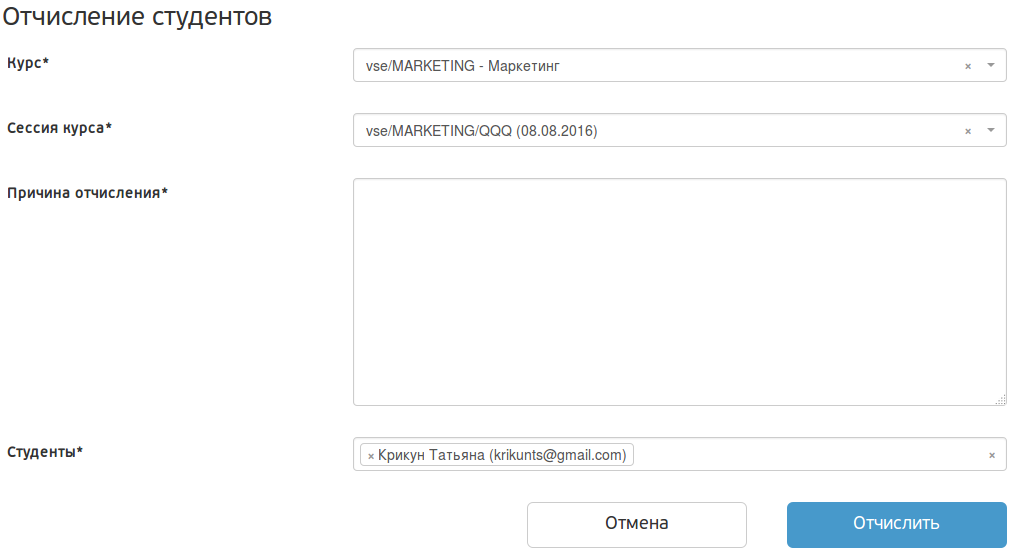
\includegraphics[width=1\linewidth]{unenroll}}
	\caption{Отчисление студентов с сессии курса}
	\label{img:student:unenroll}
\end{figure}


Для отчисления студентов необходимо:
\begin{enumerate}
	\item в выпадающем списке с автодополнением выбрать курс, на который зачислены студенты 
	(описание виджета см. в подразделе~\ref{widget:autocomplete});
	\item в выпадающем списке с автодополнением выбрать конкретную сессию этого курса 
	(описание виджета см. в подразделе~\ref{widget:autocomplete});
	\item указать причину отчисления в текстовом поле; 
	\item выбрать одного или нескольких студентов из числа уже зарегистрированных пользователей на Платформе при помощи 
	виджета выпадающего списка с автодополнением с возможностью множественного выбора 
	(описание виджета см. в подразделе~\ref{widget:autocomplete_with_multiselect}). 
\end{enumerate}

После выбора курса в выпадающем списке сессий будут перечислены только сессии выбранного курса, 
а после выбора сессии курса в списке студентов будут перечислены только студенты, 
которые были зачислены на выбранную сессию.


После заполнения всех полей необходимо нажать на кнопку \quotes{Отчислить}.

\subsection{Изменение режима прохождения сессии курса студентами}
Внешний вид формы изменения режима прохождения студентами сессии курса представлен на рис.~\ref{img:student:change_mode}.


\begin{figure}[H]
	\center{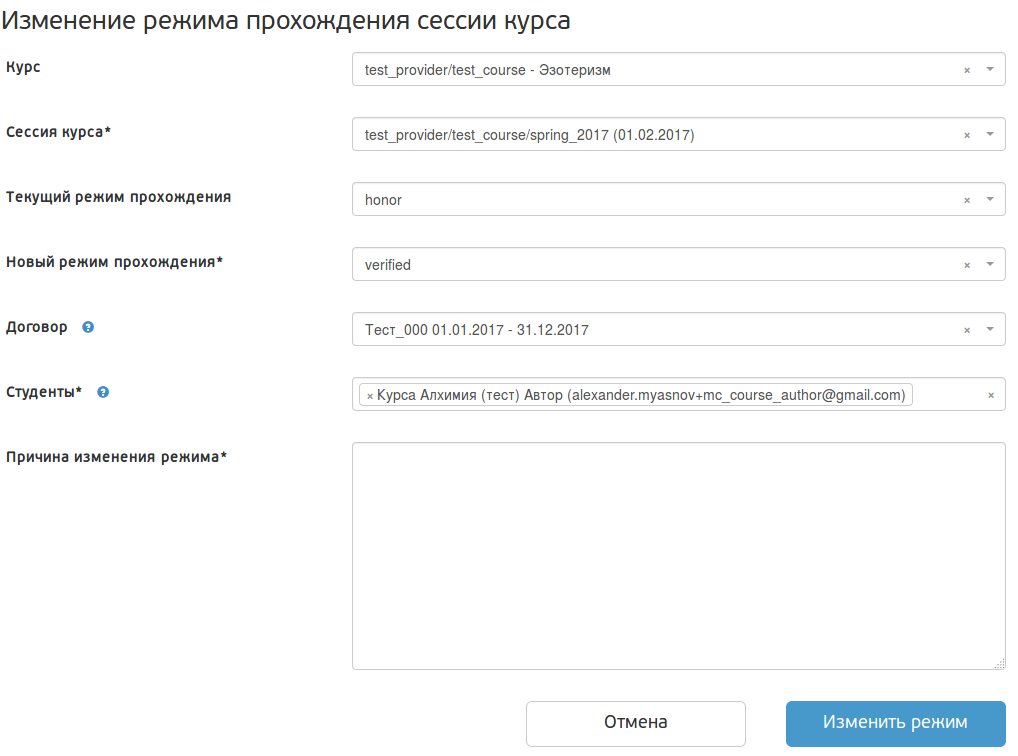
\includegraphics[width=1\linewidth]{change_mode}}
	\caption{Изменения режима прохождения студентами сессии курса}
	\label{img:student:change_mode}
\end{figure}

Для изменения режима прохождения студентами сессии курса необходимо:
\begin{enumerate}
	\item в выпадающем списке с автодополнением выбрать курс, на который зачислены студенты 
	(описание виджета см. в подразделе~\ref{widget:autocomplete});
	\item в выпадающем списке с автодополнением выбрать конкретную сессию этого курса 
	(описание виджета см. в подразделе~\ref{widget:autocomplete});
	\item в выпадающем списке с автодополнением выбрать новый режим прохождения среди доступных в рамках выбранной сессии 
	(описание виджета см. в подразделе~\ref{widget:autocomplete});
	\item опционально можно в выпадающем списке с автодополнением выбрать договор с вузом"=потребителем, 
	по которому осуществляется зачисление студентов (описание виджета см. в подразделе~\ref{widget:autocomplete});
	\item выбрать одного или нескольких студентов из числа уже зарегистрированных пользователей на Платформе при помощи 
	виджета выпадающего списка с автодополнением с возможностью множественного выбора 
	(описание виджета см. в подразделе~\ref{widget:autocomplete_with_multiselect}). 
\end{enumerate}

Изначально поля выбора договора и студентов неактивны, они активируются только после выбора сессии курса.
После выбора курса в выпадающем списке сессий будут перечислены только сессии выбранного курса, 
а в списке договоров "--- только договоры, заключенные для этого курса.
После выбора нового режима прохождения в списке студентов будут перечислены только студенты, 
которые были зачислены на выбранную сессию курса с режимом прохождения, отличным от выбранного.
В случае выбора режима <<verified>> (с подтверждением личности), поле <<договор>> становится обязательным для заполнения.


\subsection{Зачисление студентов на сессию курса списком}
Внешний вид формы зачисления студентов на сессию курса списком представлен на рис.~\ref{img:student:mass_enroll}.

\begin{figure}[H]
	\center{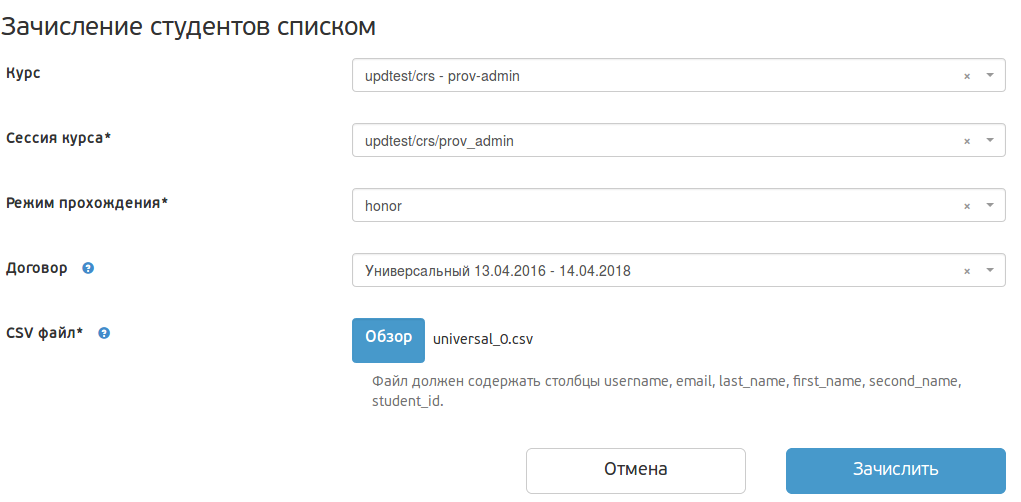
\includegraphics[width=1\linewidth]{mass_enroll}}
	\caption{Зачисление студентов на сессию курса списком}
	\label{img:student:mass_enroll}
\end{figure}

Для зачисления студентов списком необходимо:
\begin{enumerate}
	\item в выпадающем списке с автодополнением выбрать курс, который будут проходить студенты 
	(описание виджета см. в подразделе~\ref{widget:autocomplete});
	\item в выпадающем списке с автодополнением выбрать конкретную сессию этого курса 
	(описание виджета см. в подразделе~\ref{widget:autocomplete});
	\item в выпадающем списке с автодополнением выбрать один из режимов прохождения, доступных в рамках выбранной сессии 
	(описание виджета см. в подразделе~\ref{widget:autocomplete});
	\item опционально можно в выпадающем списке с автодополнением выбрать договор с вузом"=потребителем, 
	по которому осуществляется зачисление студентов (описание виджета см. в подразделе~\ref{widget:autocomplete});
	\item выбрать CSV"=файл с информацией о студентах. 
\end{enumerate}

Изначально поле выбора договора неактивно, оно активируется только после выбора сессии курса.
После выбора курса в выпадающем списке сессий будут перечислены только сессии выбранного курса, 
а в списке договоров "--- только договоры, заключенные для этого курса.
В случае выбора режима <<verified>> (с подтверждением личности), поле <<договор>> становится обязательным для заполнения. 


Для заполнения информации о студентах необходимо нажать на кнопку \quotes{Обзор} и в появившемся диалоге выбрать CSV"=файл 
с заголовком {\tt email} и данными о адресах электронной почты студентов, которых необходимо зачислить на выбранную сессию курса. 
Шаблон требуемого файла можно скачать, нажав на ссылку \quotes{Скачать шаблон}.
После заполнения всех необходимых полей необходимо нажать на кнопку \quotes{Зачислить}, 
после чего начнется загрузка файла и его обработка. 
При загрузке некорректного файла могут отобразиться следующие ошибки:
\begin{itemize}
	\item В CSV"=файле отсутствует столбец {\tt email};
	\item CSV"=файл пустой.
\end{itemize} 

При загрузке корректного файла результаты обработки отображаются в виде двух таблиц: 
первая содержит данные об успешно зачисленных студентах, 
вторая содержит данные о незачисленных студентах с указанием ошибок. 
Результат загрузки студентов представлен на рис.~\ref{img:student:mass_enroll_result}.

\begin{figure}[H]
	\center{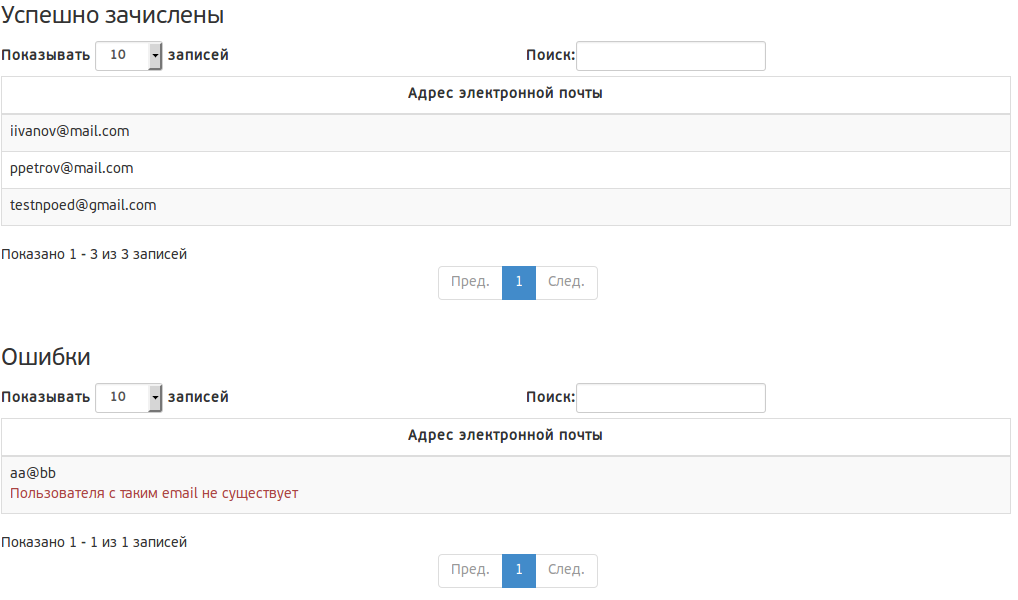
\includegraphics[width=1\linewidth]{mass_enroll_result}}
	\caption{Результат зачисления студентов на сессию курса списком}
	\label{img:student:mass_enroll_result}
\end{figure}


\subsection{Студенты вуза}

Список студентов вуза "--- это табличное представление всех студентов, ассоциированных с данным вузом.
Внешний вид списка представлен на рис.~\ref{img:student:univ_student_list}. 
Элементы управления табличными представления описаны в подразделе~\ref{sec:datatables}.
Таблица содержит следующие столбцы:
\begin{itemize}
	\item ФИО студента;
	\item все сессии курсов, на которые зачислен студент;
	\item активность;
	\item успеваемость.
\end{itemize}

\begin{figure}[H]
	\center{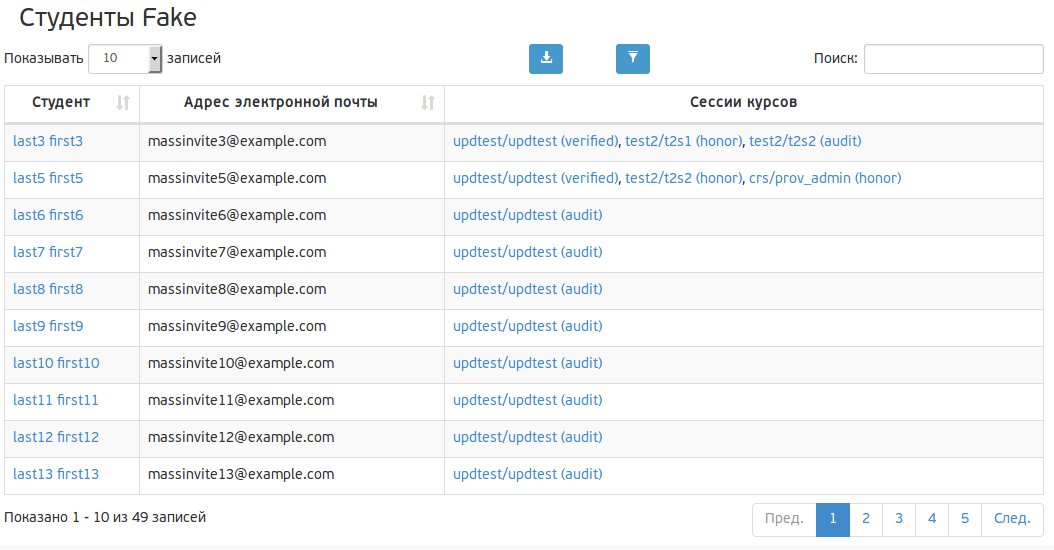
\includegraphics[width=1\linewidth]{univ_student_list}}
	\caption{Список студентов вуза}
	\label{img:student:univ_student_list}
\end{figure}

Внешний вид диалога фильтрации списка студентов представлен на рис.~\ref{img:student:univ_student_list_filter}.
Можно фильтровать список по следующим полям:
\begin{itemize}
	\item ФИО студента "--- текстовое поле;
	\item курс, на сессию которого он зачислен "--- виджет выпадающего списка с автодополнением 
	с возможностью множественного выбора (описание виджета см. в подразделе~\ref{widget:autocomplete_with_multiselect}).
\end{itemize}

 
\begin{figure}[H]
	\center{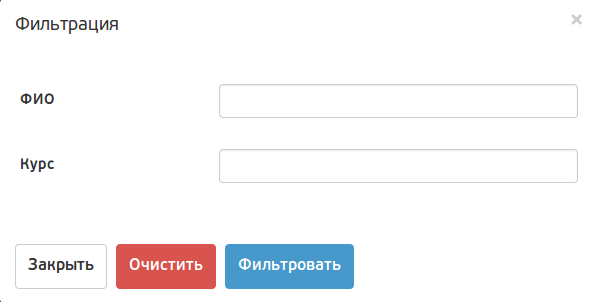
\includegraphics[height=5.5cm]{enrolled_list_filter}}
	\caption{Диалог фильтрации списка студентов вуза}
	\label{img:student:univ_student_list_filter}
\end{figure}

Каждая сессия курса в списке является ссылкой на страницу курса на сайте. 
ФИО студента является ссылкой на просмотр подробной информации о нем, 
описанной в подразделе~\ref{sec:change_mode_req_detail}.

\subsection{Подробная информация о студенте вуза} \label{sec:student_detail}
Внешний вид страницы с подробной информацией представлен на рис.~\ref{img:student:student_detail}.

\begin{figure}[H]
	\center{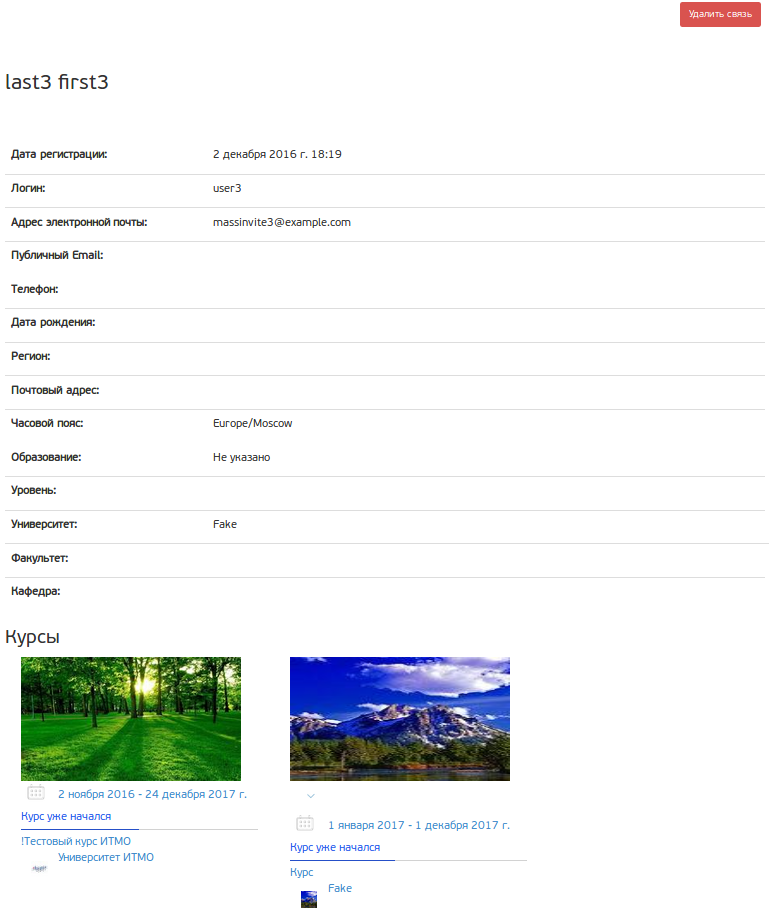
\includegraphics[width=1\linewidth]{student_detail}}
	\caption{Подробная информация о студенте}
	\label{img:student:student_detail}
\end{figure}

Для просмотра доступны следующие поля:
\begin{itemize}
	\item дата регистрации;
	\item логин;
	\item адрес электронной почты;
	\item публичный e"=mail;
	\item телефон;
	\item дата рождения;
	\item регион;
	\item почтовый адрес;
	\item часовой пояс;
	\item образование;
	\item степень;
	\item университет;
	\item факультет;
	\item кафедра;
	\item список сессий курсов, на которые записан студент.
\end{itemize}

\subsection{Заявки на зачисление}

Заявки на зачисление "--- это табличное представление заявок на зачисление студентов, 
поданных данным вузом в качестве вуза"=потребителя. 
Элементы управления табличными представления описаны в подразделе~\ref{sec:datatables}.
Внешний вид списка представлен на рис.~\ref{img:student:enroll_req_list}. 

\begin{figure}[H]
	\center{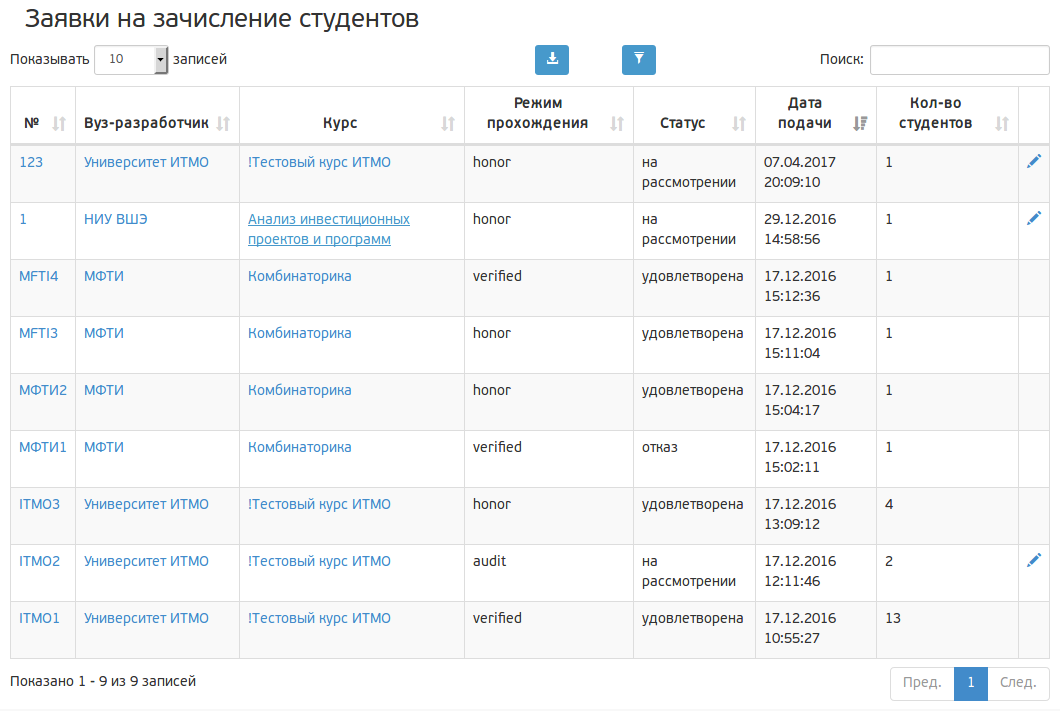
\includegraphics[width=1\linewidth]{enroll_req_list}}
	\caption{Список заявок на зачисление}
	\label{img:student:enroll_req_list}
\end{figure}

Таблица содержит следующие столбцы:
\begin{itemize}
	\item номер заявки;
	\item вуз"=разработчик;
	\item курс;
	\item режим прохождения;
	\item статус;
	\item дата подачи;
	\item количество студентов в заявке.
\end{itemize}

Внешний вид диалога фильтрации списка заявок представлен на рис.~\ref{img:student:enroll_req_list_filter}.
Можно фильтровать список по следующим параметрам:
\begin{itemize}
	\item вуз"=разработчик "--- виджет выпадающего списка с автодополнением с возможностью множественного выбора 
	(описание виджета см. в подразделе~\ref{widget:autocomplete_with_multiselect});
	\item курс "--- виджет выпадающего списка с автодополнением с возможностью множественного выбора 
	(описание виджета см. в подразделе~\ref{widget:autocomplete_with_multiselect});
	\item режим прохождения "--- виджет выпадающего списка с автодополнением с возможностью множественного выбора 
	(описание виджета см. в подразделе~\ref{widget:autocomplete_with_multiselect});
	\item статус "--- виджет выпадающего списка с автодополнением с возможностью множественного выбора 
	(описание виджета см. в подразделе~\ref{widget:autocomplete_with_multiselect});
	\item диапазон дат подачи "--- виджеты выбора даты и времени 
	(описание виджета см. в подразделе~\ref{widget:date_time_picker});
	\item диапазон количества студентов в заявке "--- числовое поле.
\end{itemize}

\begin{figure}[H]
	\center{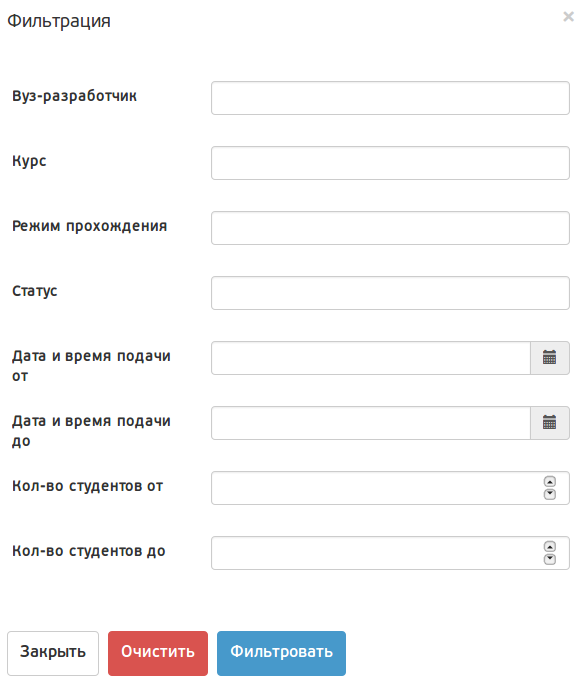
\includegraphics[height=9.1cm]{enroll_req_list_filter}}
	\caption{Диалог фильтрации списка заявок на зачисление}
	\label{img:student:enroll_req_list_filter}
\end{figure}
Номер заявки в таблице является ссылкой на страницу просмотра подробной информации о заявке, 
описанной в подразделе~\ref{sec:enroll_req_detail}.

\subsection{Подробная информация о заявке на зачисление} \label{sec:enroll_req_detail}
Внешний вид страницы с подробной информацией о заявке на зачисление представлен на рис.~\ref{img:student:enroll_req_detail}.
\begin{figure}[H]
	\center{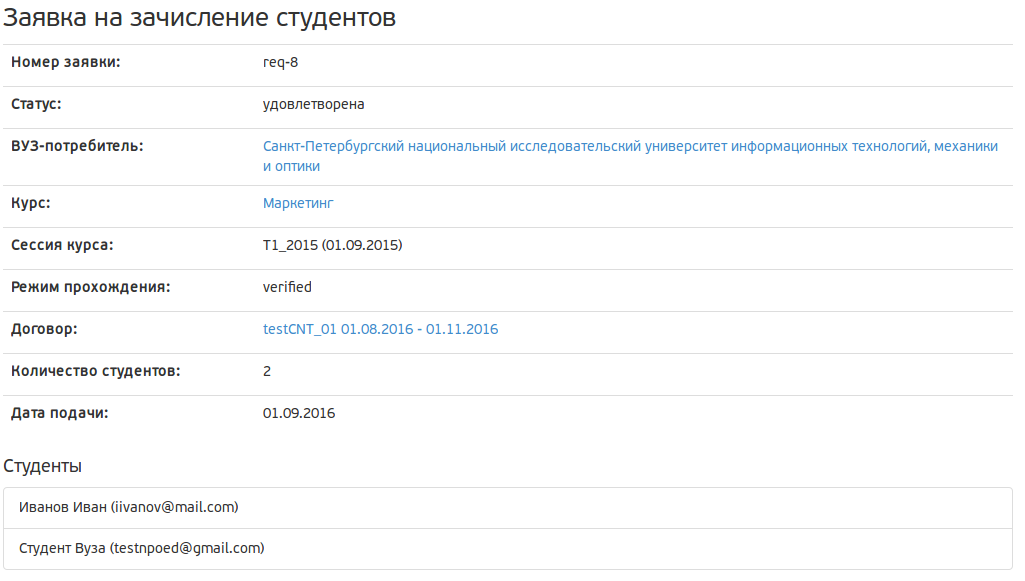
\includegraphics[height=9.1cm]{enroll_req_detail}}
	\caption{Подробная информация о заявке на зачисление}
	\label{img:student:enroll_req_detail}
\end{figure}

Для просмотра доступны следующие поля:
\begin{itemize}
	\item номер заявки;
	\item статус;
	\item причина отклонения (если есть);
	\item вуз"=потребитель;
	\item курс;
	\item сессия курса;
	\item режим прохождения;
	\item договор с вузом"=разработчиком;
	\item количество студентов в заявке;
	\item дата подачи заявки;
	\item список студентов;
\end{itemize}

Если заявка находится в состоянии \quotes{на рассмотрении}, на странице подробностей 
отображается кнопка перехода в режим редактирования заявки. \vcenteredinclude[height=25px]{edit}


Если на страницу заявки в состоянии \quotes{на рассмотрении} заходит администратор вуза"=поставщика, 
указанного в ней, для него доступны кнопки \quotes{Принять заявку} и \quotes{Отклонить заявку}, 
представленные на рис.~\ref{img:student:req_detail_buttons}.
\begin{figure}[H]
	\center{
\includegraphics[height=1cm]{req_detail_buttons}}
	\caption{Кнопки смены состояния заявки}
	\label{img:student:req_detail_buttons}
\end{figure}

При нажатии на кнопку \quotes{Принять заявку} студенты из заявки зачисляются на указанную в ней сессию курса 
с указанным режимом прохождения, а статус заявки изменяется на \quotes{удовлетворена}.

Существует несколько причин, по которым принять заявку нельзя и кнопка \quotes{Принять заявку} не показывается:
\begin{itemize}
	\item невозможно зачислить студентов на завершенную сессию курса;
	\item количество студентов в заявке превышает свободное количество студентов по договору.
\end{itemize}

При нажатии на кнопку \quotes{Отклонить заявку} появляется диалог для указания причины отказа, 
представленный на рис.~\ref{img:student:req_detail_decline}
\begin{figure}[H]
	\center{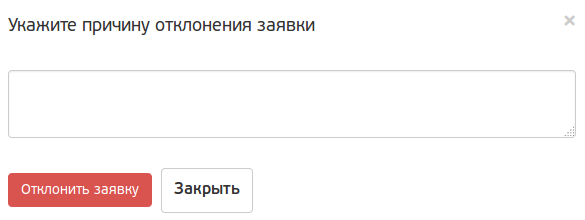
\includegraphics[height=4cm]{req_detail_decline}}
	\caption{Диалог указания причины отказа}
	\label{img:student:req_detail_decline}
\end{figure}
Для того, чтобы отклонить заявку нужно ввести причину отклонения заявки в текстовое поле диалога 
и нажать кнопку \quotes{Отклонить заявку} внизу диалога. После этого статус заявки изменяется на \quotes{отказ}.


\subsection{Заявки на изменение режима прохождения сессии курса}

Заявки на изменение режима прохождения сессии курса "--- это табличное представление заявок на изменение 
режима прохождения сессии курса, поданных данным вузом в качестве вуза"=потребителя. 
Элементы управления табличными представления описаны в подразделе~\ref{sec:datatables}.
Внешний вид списка представлен на рис.~\ref{img:student:change_mode_req_list}. 

\begin{figure}[H]
	\center{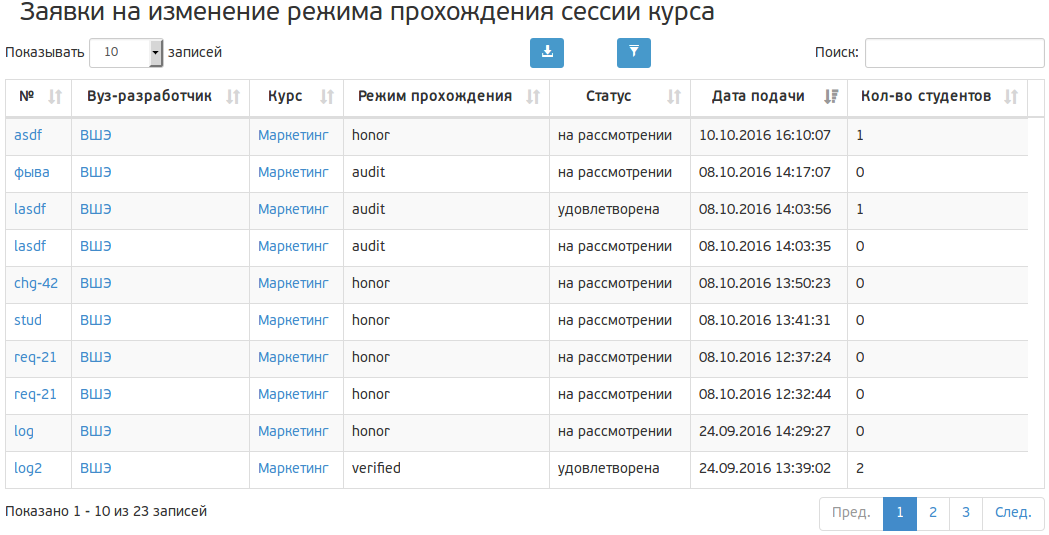
\includegraphics[width=1\linewidth]{change_mode_req_list}}
	\caption{Список заявок на изменение режима прохождения сессии курса}
	\label{img:student:change_mode_req_list}
\end{figure}

Таблица содержит следующие столбцы:
\begin{itemize}
	\item номер заявки;
	\item вуз"=разработчик;
	\item курс;
	\item режим прохождения;
	\item статус;
	\item дата подачи;
	\item количество студентов в заявке.
\end{itemize}

Внешний вид диалога фильтрации списка заявок представлен на рис.~\ref{img:student:change_mode_req_list_filter}.
\begin{figure}[H]
	\center{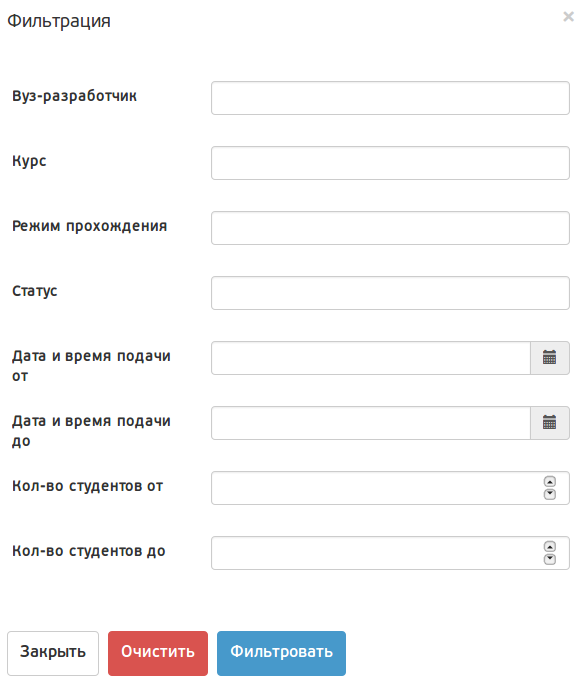
\includegraphics[height=9.1cm]{enroll_req_list_filter}}
	\caption{Диалог фильтрации списка заявок на изменение режима прохождения сессии курса}
	\label{img:student:change_mode_req_list_filter}
\end{figure}

Можно фильтровать список по следующим параметрам:
\begin{itemize}
	\item вуз"=разработчик "--- виджет выпадающего списка с автодополнением с возможностью множественного выбора 
	(см. подраздел~\ref{widget:autocomplete_with_multiselect});
	\item курс "--- виджет выпадающего списка с автодополнением с возможностью множественного выбора 
	(см. подраздел~\ref{widget:autocomplete_with_multiselect});
	\item режим прохождения "--- виджет выпадающего списка с автодополнением с возможностью множественного выбора 
	(см. подраздел~\ref{widget:autocomplete_with_multiselect});
	\item статус "--- виджет выпадающего списка с автодополнением с возможностью множественного выбора 
	(см. подраздел~\ref{widget:autocomplete_with_multiselect});
	\item диапазон дат подачи "--- виджеты выбора даты и времени 
	(см. подраздел~\ref{widget:date_time_picker});
	\item диапазон количества студентов в заявке "--- числовое поле.
\end{itemize}

Номер заявки в таблице является ссылкой на страницу просмотра подробной информации о заявке, 
описанной в подразделе~\ref{sec:change_mode_req_detail}.

\subsection{Подробная информация о заявке на изменение режима прохождения сессии курса} 
\label{sec:change_mode_req_detail}

Внешний вид страницы с подробной информацией о заявке на изменение режима прохождения сессии курса представлен 
на рис.~\ref{img:student:change_mode_req_detail}.
\begin{figure}[H]
	\center{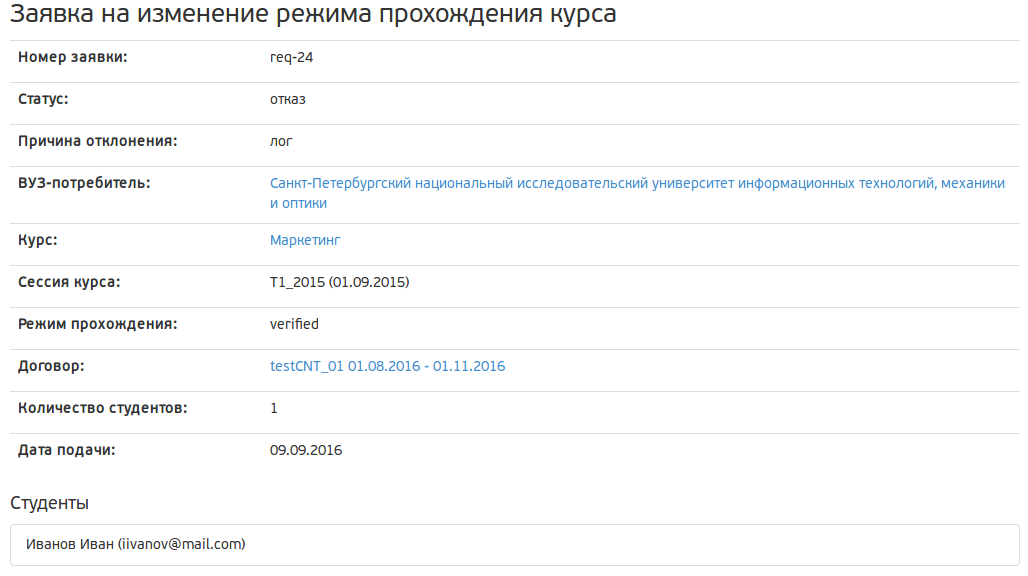
\includegraphics[height=9.1cm]{change_mode_req_detail}}
	\caption{Подробная информация о заявке на изменение режима прохождения сессии курса}
	\label{img:student:change_mode_req_detail}
\end{figure}

Для просмотра доступны следующие поля:
\begin{itemize}
	\item номер заявки;
	\item статус;
	\item причина отклонения (если есть);
	\item вуз"=потребитель;
	\item курс;
	\item сессия курса;
	\item режим прохождения;
	\item договор с вузом"=разработчиком;
	\item количество студентов в заявке;
	\item дата подачи заявки;
	\item список студентов.
\end{itemize}

Если заявка находится в состоянии \quotes{на рассмотрении}, на странице подробностей 
отображается кнопка перехода в режим редактирования заявки. \vcenteredinclude[height=25px]{edit}

Если на страницу заявки в состоянии \quotes{на рассмотрении} заходит администратор вуза"=поставщика, 
указанного в ней, для него доступны кнопки \quotes{Принять заявку} и \quotes{Отклонить заявку}, 
представленные на рис.~\ref{img:student:change_mode_req_detail_buttons}.
\begin{figure}[H]
	\center{
\includegraphics[height=1cm]{req_detail_buttons}}
	\caption{Кнопки смены состояния заявки}
	\label{img:student:change_mode_req_detail_buttons}
\end{figure}

При нажатии на кнопку \quotes{Принять заявку} студенты из заявки зачисляются на указанную в ней сессию курса 
с указанным режимом прохождения, а статус заявки изменяется на \quotes{удовлетворена}.

При нажатии на кнопку \quotes{Отклонить заявку} появляется диалог для указания причины отказа, 
представленный на рис.~\ref{img:student:change_mode_req_detail_decline}
\begin{figure}[H]
	\center{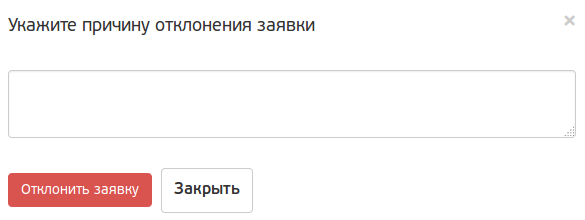
\includegraphics[height=4cm]{req_detail_decline}}
	\caption{Диалог указания причины отказа}
	\label{img:student:change_mode_req_detail_decline}
\end{figure}
Для того, чтобы отклонить заявку нужно ввести причину отклонения заявки в текстовое поле диалога 
и нажать кнопку \quotes{Отклонить заявку} внизу диалога. После этого статус заявки изменяется на \quotes{отказ}.


\subsection{Создание заявки на зачисление}
Внешний вид формы создания заявки на зачисления студентов представлен на рис.~\ref{img:student:enroll_req_create}.

\begin{figure}[H]
	\center{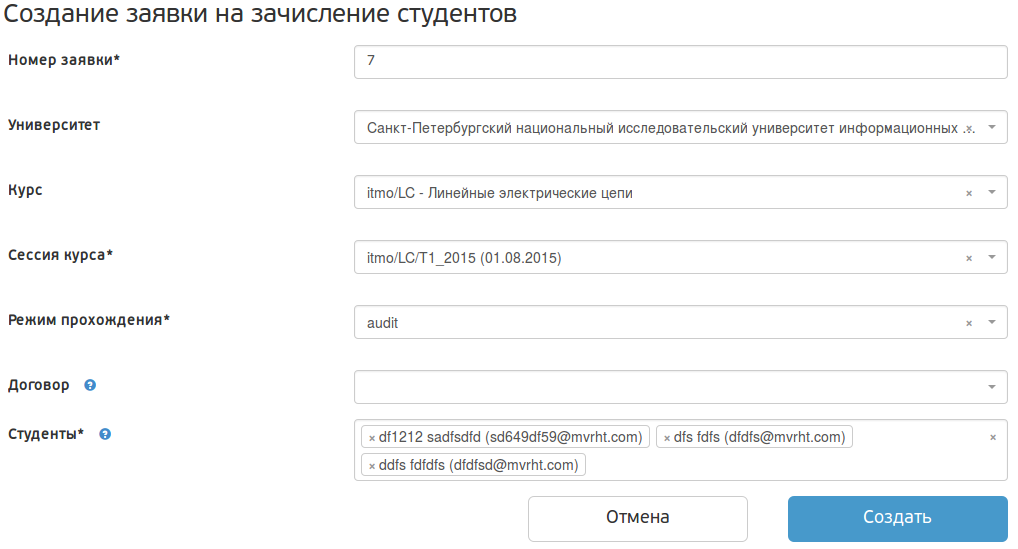
\includegraphics[width=1\linewidth]{enroll_req_create}}
	\caption{Создание заявки на зачисление студентов}
	\label{img:student:enroll_req_create}
\end{figure}

Для создания заявки на зачисление студентов необходимо:
\begin{enumerate}
	\item задать номер заявки в текстовом поле;
	\item в выпадающем списке с автодополнением выбрать вуз"=поставщик курса
	(описание виджета см. в подразделе~\ref{widget:autocomplete});
	\item в выпадающем списке с автодополнением выбрать курс выбранного вуза, который будут проходить студенты 
	(описание виджета см. в подразделе~\ref{widget:autocomplete});
	\item в выпадающем списке с автодополнением выбрать конкретную сессию этого курса 
	(описание виджета см. в подразделе~\ref{widget:autocomplete});
	\item в выпадающем списке с автодополнением выбрать один из режимов прохождения, доступных в рамках выбранной сессии 
	(описание виджета см. в подразделе~\ref{widget:autocomplete});
	\item опционально можно в выпадающем списке с автодополнением выбрать договор с выбранным вузом"=поставщиком, 
	по которому осуществляется зачисление студентов (описание виджета см. в подразделе~\ref{widget:autocomplete});
	\item выбрать одного или нескольких студентов из числа уже зарегистрированных на Платформе студентов данного вуза 
	при помощи виджета выпадающего списка с автодополнением с возможностью множественного выбора 
	(описание виджета см. в подразделе~\ref{widget:autocomplete_with_multiselect}). 
\end{enumerate}


Изначально поля выбора договора и студентов неактивны, они активируются только после выбора сессии курса.
После выбора вуза"=поставщика в выпадающем списке курсов будут перечислены только курсы, предоставляемые этим вузом.
После выбора курса в выпадающем списке сессий будут перечислены только сессии выбранного курса, 
а в списке договоров "--- только договоры, заключенные данным вузом с вузом"=разработчиком для этого курса.
После выбора сессии курса в списке студентов будут перечислены только те студенты данного вуза,
которые еще не зачислены на выбранную сессию курса.
В случае выбора режима <<verified>> (с подтверждением личности), поле <<договор>> становится обязательным для заполнения. 


В случае, если заполнено поле договора с вузом"=потребителем и количество свободных мест по договору меньше, 
чем количество выбранных для зачисления студентов, система выдаст предупреждение 
(рис.~\ref{img:student:enroll_req_create_student_error}), но на возможность зачисления студентов оно не влияет.

\begin{figure}[H]
	\center{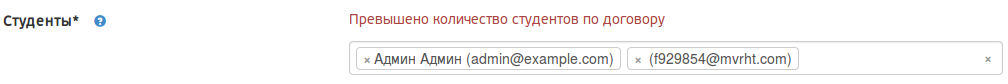
\includegraphics[width=1\linewidth]{enroll_student_error}}
	\caption{Превышение количества студентов по договору.}
	\label{img:student:enroll_req_create_student_error}
\end{figure}

После заполнения всех полей необходимо нажать на кнопку \quotes{Создать}.

\subsection{Создание заявки на зачисление списком}
Внешний вид формы создания заявки на зачисления студентов списком представлен на рис.~\ref{img:student:mass_enroll_req_create}.

\begin{figure}[H]
	\center{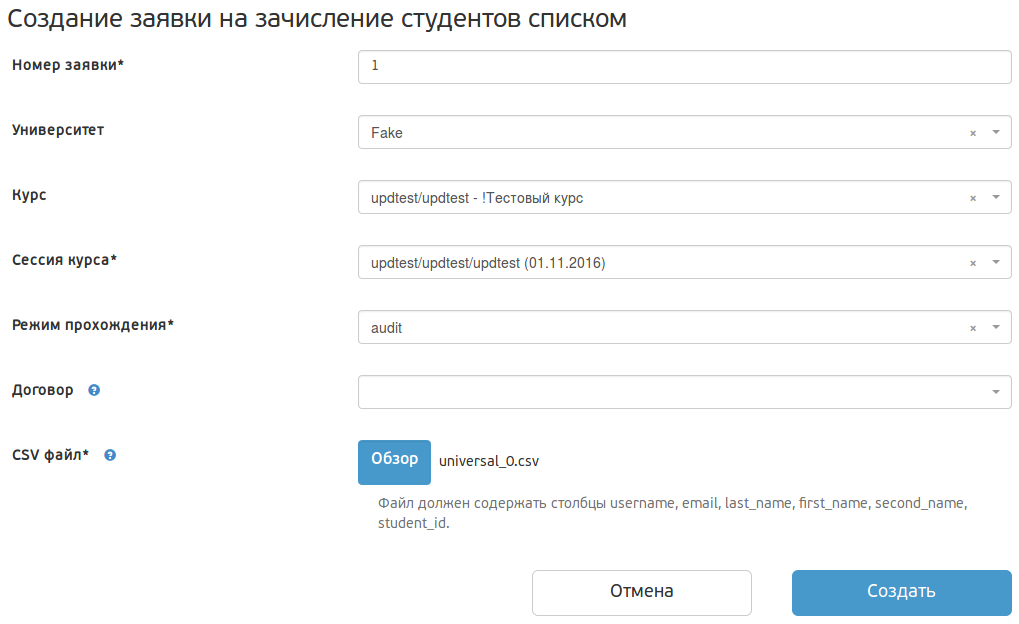
\includegraphics[width=1\linewidth]{mass_enroll_req_create}}
	\caption{Создание заявки на зачисление студентов списком}
	\label{img:student:mass_enroll_req_create}
\end{figure}

Для создания заявки на зачисление студентов списком необходимо:
\begin{enumerate}
	\item задать номер заявки в текстовом поле;
	\item в выпадающем списке с автодополнением выбрать вуз"=поставщик курса
	(описание виджета см. в подразделе~\ref{widget:autocomplete});
	\item в выпадающем списке с автодополнением выбрать курс выбранного вуза, который будут проходить студенты 
	(описание виджета см. в подразделе~\ref{widget:autocomplete});
	\item в выпадающем списке с автодополнением выбрать конкретную сессию этого курса 
	(описание виджета см. в подразделе~\ref{widget:autocomplete});
	\item в выпадающем списке с автодополнением выбрать один из режимов прохождения, доступных в рамках выбранной сессии 
	(описание виджета см. в подразделе~\ref{widget:autocomplete});
	\item опционально можно в выпадающем списке с автодополнением выбрать договор с выбранным вузом"=поставщиком, 
	по которому осуществляется зачисление студентов (описание виджета см. в подразделе~\ref{widget:autocomplete});
	\item выбрать CSV"=файл с информацией о студентах. 
\end{enumerate}


Изначально поле выбора договора неактивно, оно активируется только после выбора сессии курса.
После выбора вуза"=поставщика в выпадающем списке курсов будут перечислены только курсы, предоставляемые этим вузом.
После выбора курса в выпадающем списке сессий будут перечислены только сессии выбранного курса, 
а в списке договоров "--- только договоры, заключенные данным вузом с вузом"=разработчиком для этого курса.
В случае выбора режима <<verified>> (с подтверждением личности), поле <<договор>> становится обязательным для заполнения. 

Для заполнения информации о студентах необходимо нажать на кнопку \quotes{Обзор} и в появившемся диалоге выбрать CSV"=файл 
с заголовком {\tt email} и данными об адресах электронной почты студентов, которых необходимо зачислить на выбранную сессию курса. 
Шаблон требуемого файла можно скачать, нажав на ссылку \quotes{Скачать шаблон}.
После заполнения всех необходимых полей необходимо нажать на кнопку \quotes{Создать}, 
после чего начнется загрузка файла и его обработка. 


При загрузке некорректного файла могут отобразиться следующие ошибки:
\begin{itemize}
	\item в CSV"=файле отсутствует столбец {\tt email};
	\item CSV"=файл пустой.
\end{itemize} 

При загрузке корректного файла результаты обработки отображаются в виде двух таблиц: 
первая содержит данные об успешно добавленных в заявку студентах, 
вторая содержит данные о не добавленных  в заявку студентах с указанием ошибок. 
Также появляется сообщение об успешном создании заявки со ссылкой на страницу с подробной информацией о новой заявке.
Страница подробной информации о заявке описана в подразделе~\ref{sec:enroll_req_detail}.
Результат загрузки студентов представлен на рис.~\ref{img:student:mass_enroll_req_create_result}.

\begin{figure}[H]
	\center{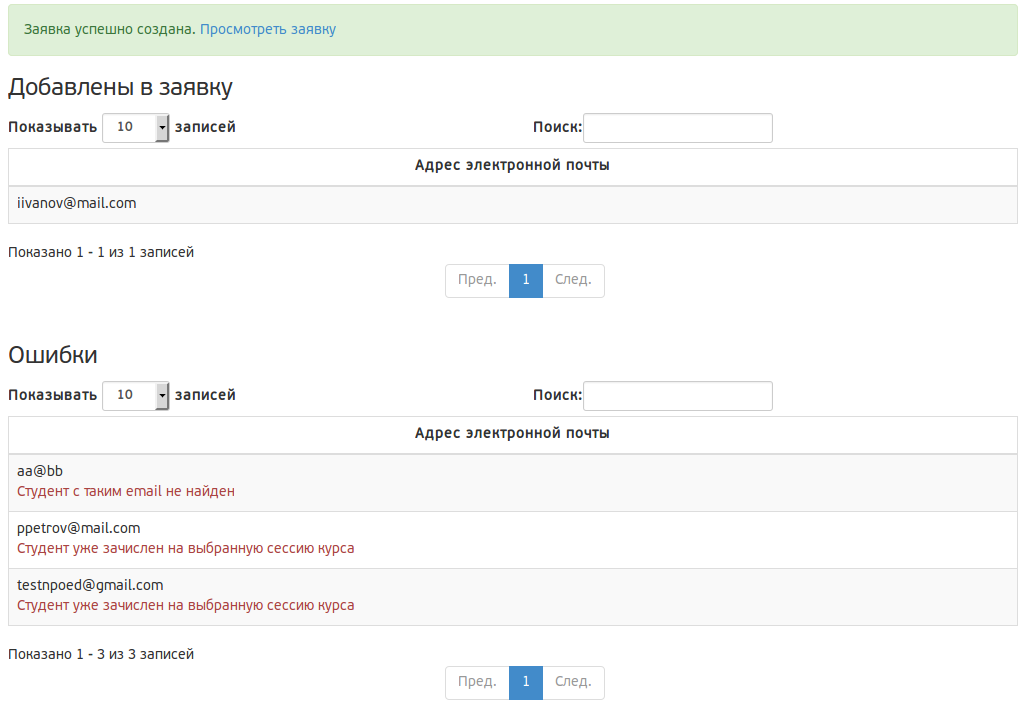
\includegraphics[width=1\linewidth]{mass_enroll_req_create_result}}
	\caption{Результат создания заявки на зачисление студентов списком }
	\label{img:student:mass_enroll_req_create_result}
\end{figure}

Если в результате обработки файла в нем не оказалось ни одного студента без ошибок, то 
система выдает сообщение \quotes{Необходимо указать хотя бы одного студента в заявке}, а новая заявка не создается.

\subsection{Создание заявки на изменение режима прохождения сессии курса студентами}

Внешний вид формы создания заявки на изменение режима прохождения сессии курса студентами
представлен на рис.~\ref{img:student:change_mode_req_create}.

\begin{figure}[H]
	\center{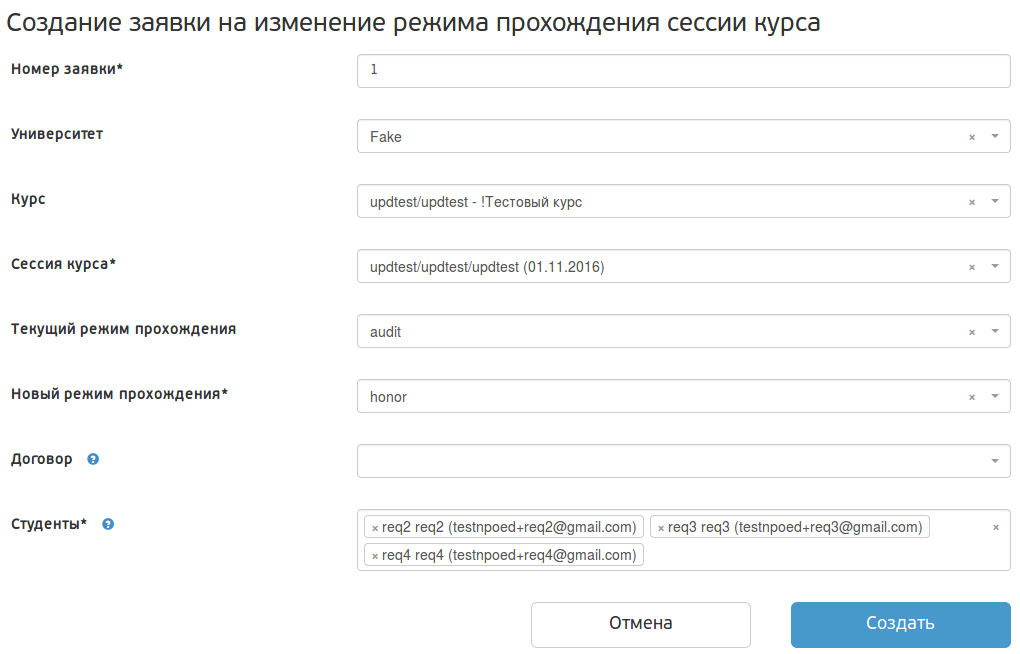
\includegraphics[width=1\linewidth]{change_mode_req_create}}
	\caption{Создание заявки на изменение режима прохождения сессии курса студентами}
	\label{img:student:change_mode_req_create}
\end{figure}

Для создания заявки на изменение режима прохождения сессии курса студентами необходимо:
\begin{enumerate}
	\item задать номер заявки в текстовом поле;
	\item в выпадающем списке с автодополнением выбрать вуз"=поставщик курса
	(описание виджета см. в подразделе~\ref{widget:autocomplete});
	\item в выпадающем списке с автодополнением выбрать курс выбранного вуза, который будут проходить студенты 
	(описание виджета см. в подразделе~\ref{widget:autocomplete});
	\item в выпадающем списке с автодополнением выбрать конкретную сессию этого курса 
	(описание виджета см. в подразделе~\ref{widget:autocomplete});
	\item в выпадающем списке с автодополнением выбрать новый режим прохождения из доступных в рамках выбранной сессии 
	(описание виджета см. в подразделе~\ref{widget:autocomplete});
	\item опционально можно в выпадающем списке с автодополнением выбрать договор с выбранным вузом"=поставщиком, 
	по которому осуществляется зачисление студентов (описание виджета см. в подразделе~\ref{widget:autocomplete});
	\item выбрать одного или нескольких студентов из числа уже зарегистрированных на Платформе студентов данного вуза 
	при помощи виджета выпадающего списка с автодополнением с возможностью множественного выбора 
	(описание виджета см. в подразделе~\ref{widget:autocomplete_with_multiselect}). 
\end{enumerate}


Изначально поля выбора договора и студентов неактивны, они активируются только после выбора сессии курса.
После выбора вуза"=поставщика в выпадающем списке курсов будут перечислены только курсы, предоставляемые этим вузом.
После выбора курса в выпадающем списке сессий будут перечислены только сессии выбранного курса, 
а в списке договоров "--- только договоры, заключенные данным вузом с вузом"=разработчиком для этого курса.
После выбора режима прохождения в списке студентов будут перечислены только те студенты данного вуза, 
которые были зачислены на выбранную сессию курса с режимом прохождения, отличным от выбранного.
В случае выбора режима <<verified>> (с подтверждением личности), поле <<договор>> становится обязательным для заполнения. 


В случае, если заполнено поле договора с вузом"=потребителем и количество свободных мест по договору меньше, 
чем количество выбранных для зачисления студентов, система выдаст предупреждение 
(рис.~\ref{img:student:change_mode_req_create_student_error}), но на возможность зачисления студентов оно не влияет.

\begin{figure}[H]
	\center{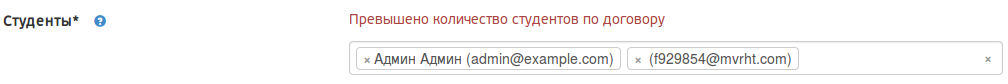
\includegraphics[width=1\linewidth]{enroll_student_error}}
	\caption{Превышение количества студентов по договору.}
	\label{img:student:change_mode_req_create_student_error}
\end{figure}

После заполнения всех полей необходимо нажать на кнопку \quotes{Создать}.

\subsection{Создание заявки на изменение режима прохождения сессии курса студентами списком}
Внешний вид формы создания заявки на изменение режима прохождения сессии курса студентами списком 
представлен на рис.~\ref{img:student:mass_change_mode_req_create}.

\begin{figure}[H]
	\center{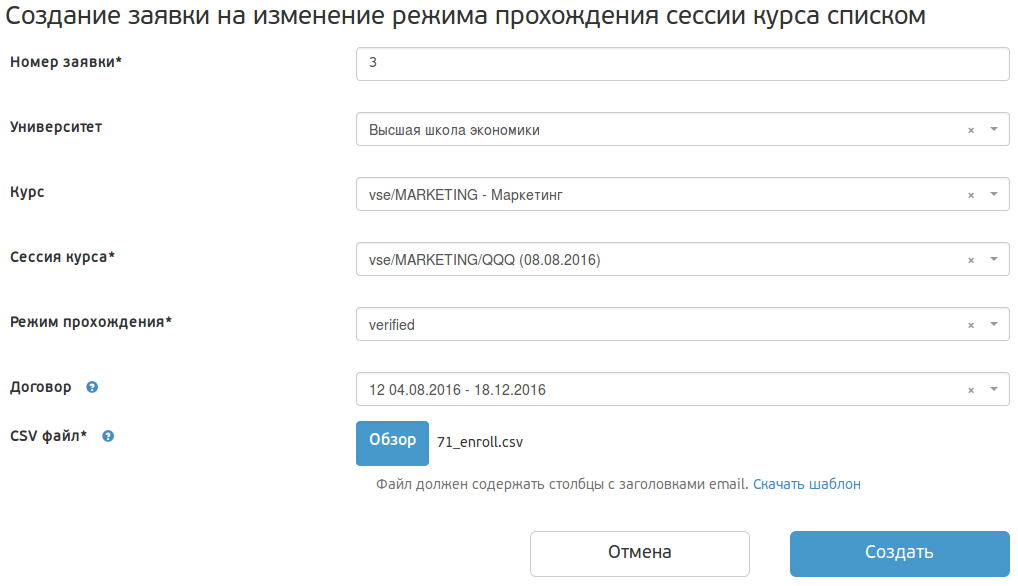
\includegraphics[width=1\linewidth]{mass_change_mode_req_create}}
	\caption{Создание заявки на изменение режима прохождения сессии курса студентами списком}
	\label{img:student:mass_change_mode_req_create}
\end{figure}

Для создания заявки на изменение режима прохождения сессии курса студентами списком необходимо:
\begin{enumerate}
	\item задать номер заявки в текстовом поле;
	\item в выпадающем списке с автодополнением выбрать вуз"=поставщик курса
	(описание виджета см. в подразделе~\ref{widget:autocomplete});
	\item в выпадающем списке с автодополнением выбрать курс выбранного вуза, который будут проходить студенты 
	(описание виджета см. в подразделе~\ref{widget:autocomplete});
	\item в выпадающем списке с автодополнением выбрать конкретную сессию этого курса 
	(описание виджета см. в подразделе~\ref{widget:autocomplete});
	\item в выпадающем списке с автодополнением выбрать новый режим прохождения из доступных в рамках выбранной сессии 
	(описание виджета см. в подразделе~\ref{widget:autocomplete});
	\item опционально можно в выпадающем списке с автодополнением выбрать договор с выбранным вузом"=поставщиком, 
	по которому осуществляется зачисление студентов (описание виджета см. в подразделе~\ref{widget:autocomplete});
	\item выбрать CSV"=файл с информацией о студентах.
\end{enumerate}

Изначально поле выбора договора неактивно, оно активируется только после выбора сессии курса.
После выбора вуза"=поставщика в выпадающем списке курсов будут перечислены только курсы, предоставляемые этим вузом.
После выбора курса в выпадающем списке сессий будут перечислены только сессии выбранного курса, 
а в списке договоров "--- только договоры, заключенные данным вузом с вузом"=разработчиком для этого курса.
В случае выбора режима <<verified>> (с подтверждением личности), поле <<договор>> становится обязательным для заполнения. 

Для заполнения информации о студентах необходимо нажать на кнопку \quotes{Обзор} и в появившемся диалоге выбрать CSV"=файл 
с заголовком {\tt email} и данными о адресах электронной почты студентов, которых необходимо зачислить на выбранную сессию курса. 
Шаблон требуемого файла можно скачать, нажав на ссылку \quotes{Скачать шаблон}.
После заполнения всех необходимых полей необходимо нажать на кнопку \quotes{Создать}, 
после чего начнется загрузка файла и его обработка. При загрузке некорректного файла могут отобразиться следующие ошибки:
\begin{itemize}
	\item В CSV"=файле отсутствует столбец {\tt email};
	\item CSV"=файл пустой.
\end{itemize} 

При загрузке корректного файла результаты обработки отображаются в виде двух таблиц: 
первая содержит данные об успешно добавленных в заявку студентах, 
вторая содержит данные о не добавленных в заявку студентах с указанием ошибок. 
Также появляется сообщение об успешном создании заявки со ссылкой на страницу с подробной информацией о новой заявке.
Страница подробной информации о заявке описана в подразделе~\ref{sec:change_mode_req_detail}.
Результат загрузки студентов представлен на рис.~\ref{img:student:mass_change_mode_req_create_result}.

\begin{figure}[H]
	\center{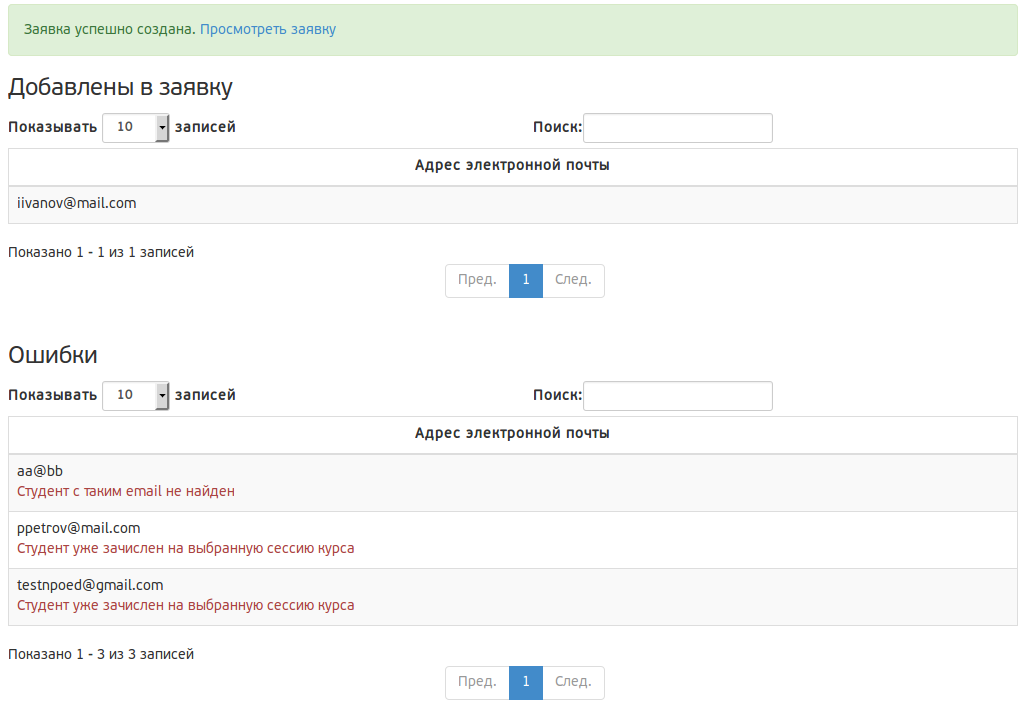
\includegraphics[width=1\linewidth]{mass_enroll_req_create_result}}
	\caption{Результат создания заявки на изменение режима прохождения сессии курса студентами списком}
	\label{img:student:mass_change_mode_req_create_result}
\end{figure}

Если в результате обработки файла в нем не оказалось ни одного студента без ошибок, то 
система выдает сообщение \quotes{Необходимо указать хотя бы одного студента в заявке}, а новая заявка не создается.
